


\tikzset{every picture/.style={line width=0.75pt}} %set default line width to 0.75pt        

\begin{tikzpicture}[x=0.75pt,y=0.75pt,yscale=-1,xscale=1]
%uncomment if require: \path (0,534); %set diagram left start at 0, and has height of 534

%Curve Lines [id:da3428774655789326] 
\onslide<6-7>{\draw [color={rgb, 255:red, 255; green, 0; blue, 0 }  ,draw opacity=1 ]   (253,380) .. controls (293,360) and (325,363) .. (357,387) ;}
%Curve Lines [id:da41651271023154823] 
\onslide<7>{\draw [color={rgb, 255:red, 0; green, 0; blue, 255 }  ,draw opacity=1 ]   (258,333) .. controls (298,313) and (330,316) .. (362,340) ;}
%Curve Lines [id:da3428774655789326] 
\onslide<8->{\draw [color={rgb, 255:red, 255; green, 0; blue, 0 }  ,draw opacity=1 ]   (253,380) .. controls (292,366) and (308,378) .. (301,401) ;}
%Curve Lines [id:da41651271023154823] 
\onslide<8>{\draw [color={rgb, 255:red, 0; green, 0; blue, 255 }  ,draw opacity=1 ]   (255,375) .. controls (297,361) and (326,364) .. (359,382) ;}
%Curve Lines [id:da5138180188097863] 
\onslide<8->{\draw [color={rgb, 255:red, 255; green, 0; blue, 0 }  ,draw opacity=1 ]   (301,401) .. controls (308,376) and (325,363) .. (357,387) ;}
%Shape: Ellipse [id:dp021620768392659695] 
\onslide<9->{\draw  [color={rgb, 255:red, 0; green, 0; blue, 255 }  ,draw opacity=1 ] (270,388) .. controls (270,378.06) and (286.79,370) .. (307.5,370) .. controls (328.21,370) and (345,378.06) .. (345,388) .. controls (345,397.94) and (328.21,406) .. (307.5,406) .. controls (286.79,406) and (270,397.94) .. (270,388) -- cycle ;}

% Text Node
\onslide<2,4->{\draw (278,380) node [anchor=north west][inner sep=0.75pt]    {$B_{2}$};}
\onslide<3>{\draw (278,380) node [anchor=north west][inner sep=0.75pt] [opacity=0.2  ]    {$B_{2}$};}
% Text Node
\onslide<4->{\draw (309,332) node [anchor=north west][inner sep=0.75pt]    {$B_{4}$};}
\onslide<2-3>{\draw (309,332) node [anchor=north west][inner sep=0.75pt] [opacity=0.2  ]    {$B_{4}$};}
% Text Node
\draw (278,429) node [anchor=north west][inner sep=0.75pt]    {$B_{1}$};
% Text Node
\onslide<3->{\draw (318,380) node [anchor=north west][inner sep=0.75pt]    {$B_{3}$};}
\onslide<2>{\draw (318,380) node [anchor=north west][inner sep=0.75pt] [opacity=0.2  ]    {$B_{3}$};}
% Text Node
\onslide<5->{\draw (309,287) node [anchor=north west][inner sep=0.75pt]    {$B_{5}$};}
\onslide<2-4>{\draw (309,287) node [anchor=north west][inner sep=0.75pt] [opacity=0.2  ]    {$B_{5}$};}
% Connection 1
\onslide<2,4->{\draw    (286.5,402) -- (286.5,423) ;
\draw [shift={(286.5,400)}, rotate = 90] [color={rgb, 255:red, 0; green, 0; blue, 0 }  ][line width=0.75]    (10.93,-3.29) .. controls (6.95,-1.4) and (3.31,-0.3) .. (0,0) .. controls (3.31,0.3) and (6.95,1.4) .. (10.93,3.29)   ;}
\onslide<3>{\draw [opacity=0.2  ]    (286.5,402) -- (286.5,423) ;
\draw [shift={(286.5,400)}, rotate = 90] [color={rgb, 255:red, 0; green, 0; blue, 0 },opacity=0.2  ][line width=0.75]    (10.93,-3.29) .. controls (6.95,-1.4) and (3.31,-0.3) .. (0,0) .. controls (3.31,0.3) and (6.95,1.4) .. (10.93,3.29)   ;}
% Connection 3
\onslide<4->{\draw    (294.9,374) -- (308.02,353.68) ;
\draw [shift={(309.1,352)}, rotate = 122.86] [color={rgb, 255:red, 0; green, 0; blue, 0 }  ][line width=0.75]    (10.93,-3.29) .. controls (6.95,-1.4) and (3.31,-0.3) .. (0,0) .. controls (3.31,0.3) and (6.95,1.4) .. (10.93,3.29)   ;}
\onslide<2-3>{\draw [opacity=0.2  ]    (294.9,374) -- (308.02,353.68) ;
\draw [shift={(309.1,352)}, rotate = 122.86] [color={rgb, 255:red, 0; green, 0; blue, 0 },opacity=0.2  ][line width=0.75]    (10.93,-3.29) .. controls (6.95,-1.4) and (3.31,-0.3) .. (0,0) .. controls (3.31,0.3) and (6.95,1.4) .. (10.93,3.29)   ;}
% Connection 4
\onslide<4->{\draw    (324.06,374) -- (320.31,353.97) ;
\draw [shift={(319.94,352)}, rotate = 79.38] [color={rgb, 255:red, 0; green, 0; blue, 0 }  ][line width=0.75]    (10.93,-3.29) .. controls (6.95,-1.4) and (3.31,-0.3) .. (0,0) .. controls (3.31,0.3) and (6.95,1.4) .. (10.93,3.29)   ;}
\onslide<2-3>{\draw [opacity=0.2  ]    (324.06,374) -- (320.31,353.97) ;
\draw [shift={(319.94,352)}, rotate = 79.38] [color={rgb, 255:red, 0; green, 0; blue, 0 },opacity=0.2  ][line width=0.75]    (10.93,-3.29) .. controls (6.95,-1.4) and (3.31,-0.3) .. (0,0) .. controls (3.31,0.3) and (6.95,1.4) .. (10.93,3.29)   ;}
% Connection 2
\onslide<3->{\draw    (297.11,423) -- (314.62,401.55) ;
\draw [shift={(315.89,400)}, rotate = 129.23] [color={rgb, 255:red, 0; green, 0; blue, 0 }  ][line width=0.75]    (10.93,-3.29) .. controls (6.95,-1.4) and (3.31,-0.3) .. (0,0) .. controls (3.31,0.3) and (6.95,1.4) .. (10.93,3.29)   ;}
\onslide<2>{\draw [opacity=0.2  ]    (297.11,423) -- (314.62,401.55) ;
\draw [shift={(315.89,400)}, rotate = 129.23] [color={rgb, 255:red, 0; green, 0; blue, 0 },opacity=0.2  ][line width=0.75]    (10.93,-3.29) .. controls (6.95,-1.4) and (3.31,-0.3) .. (0,0) .. controls (3.31,0.3) and (6.95,1.4) .. (10.93,3.29)   ;}
% Connection 5
\onslide<5->{\draw    (317.5,326) -- (317.5,309) ;
\draw [shift={(317.5,307)}, rotate = 90] [color={rgb, 255:red, 0; green, 0; blue, 0 }  ][line width=0.75]    (10.93,-3.29) .. controls (6.95,-1.4) and (3.31,-0.3) .. (0,0) .. controls (3.31,0.3) and (6.95,1.4) .. (10.93,3.29)   ;}
\onslide<2-4>{\draw [opacity=0.2  ]    (317.5,326) -- (317.5,309) ;
\draw [shift={(317.5,307)}, rotate = 90] [color={rgb, 255:red, 0; green, 0; blue, 0 },opacity=0.2  ][line width=0.75]    (10.93,-3.29) .. controls (6.95,-1.4) and (3.31,-0.3) .. (0,0) .. controls (3.31,0.3) and (6.95,1.4) .. (10.93,3.29)   ;}

% \draw (250,287) node [anchor=north west][inner sep=0.75pt]    {$G$};

% Text Node
\onslide<6-7>{\draw (228,350) node [anchor=north west][inner sep=0.75pt]  [font=\small,color={rgb, 255:red, 0; green, 0; blue, 0 }  ,opacity=1 ]  {$\tau =\nicefrac{1}{8}$};}
\onslide<8->{\draw (228,350) node [anchor=north west][inner sep=0.75pt]  [font=\small,color={rgb, 255:red, 0; green, 0; blue, 0 }  ,opacity=1 ]  {\o{$\tau =\nicefrac{1}{4}$}};}

% Text Node
\onslide<6-8>{\draw (337,387) node [anchor=north west][inner sep=0.75pt]  [color={rgb, 255:red, 255; green, 0; blue, 0 }  ,opacity=1 ]  {$\L$};}
\onslide<9->{\draw (345,390) node [anchor=north west][inner sep=0.75pt]  [color={rgb, 255:red, 255; green, 0; blue, 0 }  ,opacity=1 ]  {$\L$};}
% Text Node
\onslide<7>{\draw (335,338) node [anchor=north west][inner sep=0.75pt]  [color={rgb, 255:red, 0; green, 0; blue, 255 }  ,opacity=1 ]  {$\U$};}
\onslide<8->{\draw (335,355) node [anchor=north west][inner sep=0.75pt]  [color={rgb, 255:red, 0; green, 0; blue, 255 }  ,opacity=1 ]  {$\U$};}

\end{tikzpicture}
